\section{Proposed and Ongoing Work}
\subsection{Evidence-Derived Answering}
Medical VLMs can provide a correct spatial answer and a separate point that does not support it. Across the reported baselines, 9.4--15.0\% of correct answers point outside the lesion box. Evidence-Derived Answering (EDA) \citep{eda} makes the relation between a final point and a spatial answer explicit. Hanqi Jiang is first author of this work from the Lei Xing lab at Stanford, submitted to CVPR 2027.

The model first produces a point, may invoke windowing or a $2\times$ zoom, and then may re-point. A declared deterministic readout converts the final point into an answer: examples include a body midline, a TotalSegmentator lobe map, or chest-radiograph lung-zone thirds. The answer is therefore derived from the point according to the rule, although neither point correctness nor segmentation correctness follows automatically. Supervised fine-tuning uses a lesion-size zoom prior, followed by GRPO reinforcement learning with a box-aware reward and counterfactual advantage on zoom and window decision tokens. The setup includes Qwen2.5-VL-3B with LoRA and a frozen vision tower, Qwen3-VL-8B, and datasets spanning BraTS, MSD-Lung, LUNA16, MIMIC-CXR/MS-CXR, ChestX-Det, and supplementary MSD liver data.
Figure~\ref{fig:eda_method} shows the training and inference pipeline.
\begin{figure}[htbp]\centering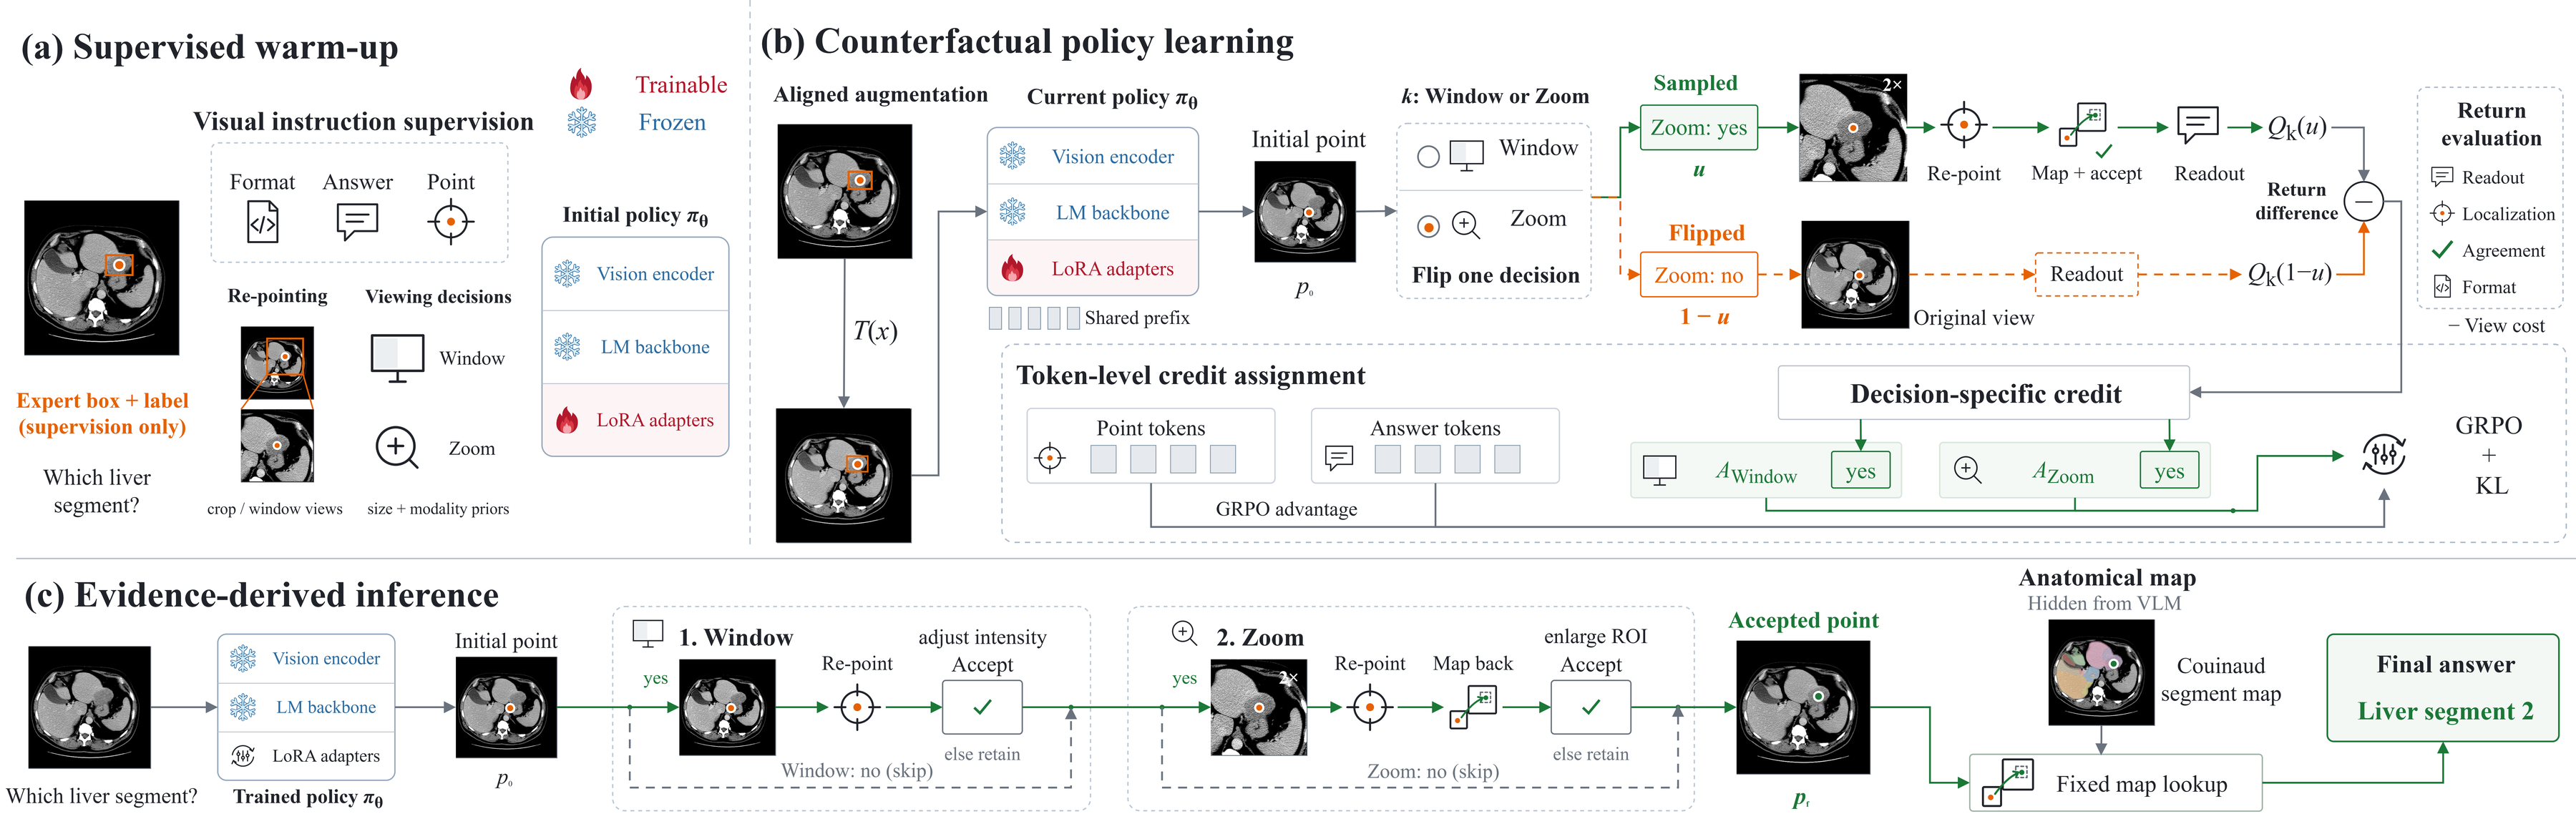
\includegraphics[width=\textwidth,height=.34\textheight,keepaspectratio]{figures/eda_method.png}\caption{EDA begins with supervised warm-up on an image and question, teaching the output format, pointing, viewing decisions, and re-pointing on window and zoom views; the expert box and label serve as supervision. Counterfactual policy learning compares sampled viewing decisions with their flipped counterparts on aligned augmentations, crediting decision tokens with the return difference and point and answer tokens with the GRPO advantage. At inference, the policy points and may window or zoom and re-point. A fixed lookup of the accepted point in an anatomical map hidden from the VLM yields the answer. Adapted from EDA Fig. 2. Source: EDA \citep{eda}.}\label{fig:eda_method}\end{figure}

On Qwen2.5-VL-3B, mean joint accuracy is 70.7\% versus 62.2\% for ViGoRL; on Qwen3-VL-8B the comparison is 82.9\% versus 74.8\%. On held-out LUNA16, EDA achieves 50.9\% versus 35.0\%. The outside-box share among correct answers is 6.8\%.

Selective zoom fires for 440 of 1,761 questions, approximately 25\%, and achieves 70.7\% versus 68.6\% with forced zoom; windowing is never called in that experiment. This measures selective perception, not end-to-end energy. Boxes are available for 251 of 2,658 patients (9.4\%); training without versus with retained boxes gives 50.1\% and 51.6\%, compared with 44.9\% for the baseline. Further work will draw final figures to replace source placeholders, add seeds and variance estimates, consider a reader study, and finalize the appendix. CVPR notification is pending; its date is TBD.

We will test the hypothesis that the declared point-to-answer readout can retain joint accuracy relative to free-form spatial answering. Evaluation will use joint accuracy and outside-box share on the training-source datasets and held-out LUNA16. We will add seeds and variance estimates to the main comparisons. Selective zoom may not generalize to unseen modalities; forced zoom provides a comparison if selective decisions fail to transfer.

\subsection{Medical Findings Are Prediction Errors}
Supervised detectors require annotations describing where and what a finding is, whereas anomaly maps may locate unusual regions without naming them. Medical Findings Are Prediction Errors (PER) \citep{per} proposes a masked-context U-Net world model trained only on normal or unlabeled scans with a heteroscedastic $\beta$-NLL objective. Peaks of smoothed precision-weighted prediction error propose candidates. A Qwen3-VL-8B LoRA verifier then names a finding through yes/no decisions. Hanqi Jiang is first author of this work from the Lei Xing lab at Stanford, submitted to CVPR 2027.
Figure~\ref{fig:per} shows candidate generation and verification.
\begin{figure}[htbp]\centering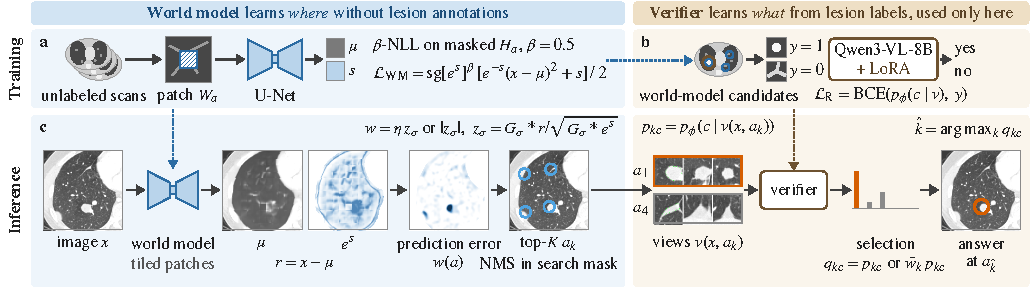
\includegraphics[width=\textwidth,height=.30\textheight,keepaspectratio]{figures/per.pdf}\caption{The world model receives an image patch with a masked region and a binary mask and predicts pixel expectations and variances. A prediction-error map combines the residual with the predicted variance, and its peaks yield candidate locations and weights within the search mask. During training, the verifier learns from world-model candidates. At inference, it scores candidate-centered views for each finding; selection uses verifier scores, with or without world-model weights, to choose an answer. Adapted from PER Fig. 2. Source: PER \citep{per}.}\label{fig:per}\end{figure}
The world model asks what image content is predictable from context. High error is a candidate signal, not a diagnosis: normal variation, acquisition artifacts, or diffuse disease may also affect prediction. The verifier supplies semantic information, so lesion labels train the verifier. Evaluation spans chest radiographs, lung and liver CT, and longitudinal CT, including ChestX-Det, LUNA16, MSD, and external datasets.

On LUNA16, PER reports 0.83/0.84 for the two sets versus 0.80/0.77 for 3D RetinaNet. Longitudinal results are 0.80/0.90 versus 0.75/0.80 for LesionLocator. ChestX-Det AUROC is 0.846, compared with 0.851 for RT-DETRv2. The candidate generator uses zero lesion labels; without the verifier, lung CT results are 0.75/0.67, while radiograph LROC is 0.083. This ablation shows the importance of the naming stage and the limits of unverified prediction error.

The lung Set 1 label-efficiency curve reports 0.69, 0.75, 0.74, and 0.76 at 5\%, 10\%, 25\%, and 50\% labels, respectively; 3D RetinaNet at 5\% is 0.61. With a lesion-annotation-free world model and the final verifier, liver results are 0.89 on MSD and 0.85 on external HCC-TACE-Seg. The appendix remains to be finalized; the CVPR notification date is TBD.

We will test whether prediction-error candidates with a verifier can match supervised detectors at low label budgets. The evaluation will compare hit rates on LUNA16, MSD, and HCC-TACE-Seg, and AUROC and LROC on ChestX-Det, alongside repeated runs and variance estimates. Diffuse findings such as effusion or edema may yield little localized error; further analysis or an extension of the candidate method will be needed if this limits detection.

\subsection{Integration and remaining work}
The dissertation will synthesize audit, control, and derivation around a common question: does the system use the evidence required by its answer? MedVIGIL tests whether broken evidence changes behavior; RAW tests whether a specific representation direction controls an answer; EDA specifies a point-to-answer relationship; PER separates candidate generation from semantic verification. These designs answer different causal questions. An explicit readout guarantees a relation to a point, whereas a learned verifier remains a component requiring independent validation.

\begin{table}[htbp]\centering\small\caption{Efficiency synthesis across the dissertation.}\label{tab:efficiency}
\begin{tabularx}{\textwidth}{l l Y}\toprule
Facet & Work & Evidence and scope \\\midrule
Parameters & HybridMED & Shared attention and feed-forward components; no quantified parameter count. \\
Auxiliary data & EGMA & Small amounts of gaze help in the reported study. \\
Energy & EG-SpikeFormer & 52.4 mJ versus ViT 81.0 mJ; not the lowest energy in its table. \\
Perception/tokens & ViThinker; EDA & 8.6 versus 16.0 tokens; selective zoom on about 25\% of questions. \\
Lesion labels & EDA; PER & Scarce boxes; normal/unlabeled world-model training. \\
Annotation & MedVIGIL & Computed volumetric probe labels; no additional per-probe annotation. \\\bottomrule\end{tabularx}\end{table}
The integrated analysis will tabulate each work's evidence-use test and resource measure within its own protocol, including Table~\ref{tab:efficiency}, and state for each research question what was shown and what remains unvalidated. It will not run new cross-system experiments or report a combined efficiency score. It will incorporate the TMI revision outcome, extend calibration to two dimensions, and pursue the volumetric reader study. The resulting account will distinguish reported experiments from proposed work and will describe limitations of cross-dataset and clinical transfer.
